\documentclass[12pt, oneside, a4paper]{article}
\usepackage[utf8]{inputenc}
\usepackage[margin=1in]{geometry}
\usepackage{amsfonts, amsmath, amssymb}
\usepackage[none]{hyphenat}
\usepackage{fancyhdr}
\usepackage{graphicx}
\usepackage{float}
\usepackage[nottoc, notlot, notlof]{tocbibind}
\usepackage{xcolor}
\graphicspath{ {figures/} }
\pagenumbering{arabic}



\pagestyle{fancy}
\fancyhead{}
\fancyfoot{}
\fancyhead[C]{}
\fancyfoot[C]{\thepage}


\begin{document}
%\begin{titlepage}
\begin{center}
    \vspace{0.1cm}
    \begin{Large}\textbf{Securing Online Transactions}\end{Large}\\
    \vspace{1cm}\begin{large}
    \textit{A project submitted in partial fulfillment of the\\
    Requirements for the award of the degree of}\\
    \vspace{0.8cm}
    \textbf{Bachelor of Technology\\ in}\\
    \textbf{\colorbox{yellow}{COMPUTER SCIENCE AND ENGINEERING}}\\
    \vspace{0.6cm}
    
\includegraphics[width=0.3\textwidth]{Clg_logo.png}\\
    \vspace{1cm}
    \line(1,0){400}\\\vspace{0.3cm}
    Submitted by:\\
    \textbf{Mr. Harsh Bokan}\\Rol No.: 12011009\\
    \vspace{0.5cm}
    \line(1,0){150}\\
    \vspace{0.5cm}
    Supervised by:\\
    \textbf{Dr. Mukesh Mann}\\
    Assistant Professor\\
    \line(1,0){400}\\
    \vspace{2cm}
    \textbf{INDIAN INSTITUTE OF INFORMATION TECHNOLOGY,\\
    SONEPAT -131021, HARYANA, INDIA}\\\end{large}
\end{center}
\thispagestyle{empty}
%\end{titlepage}
\pagebreak
%2nd Page
\begin{center}
    \begin{Large}\textbf{ACKNOWLEDGEMENT}\end{Large}
\end{center}\\
\vspace{1cm}
I would like to extend my sincere thanks to Dr Mukesh Mann for providing us with the glorious opportunity to work on the magnificent project Securing Online Transactions and for their precious assistance at every juncture of our journey in bringing this project to reality. I find myself lucky to be the recipient of his advice and encouragement. 

I cannot ever I think, succeed in verbalising the support and inspiration bestowed upon me by my parents who despite their busy schedules never passed over any moment where they could succour me. I am very grateful for their highly cherished support during this project.

I consider myself lucky to have secured a chance to make this project as it imparted a great deal of knowledge about real life problems and the methods to approach and finally attempt to solve them. I learned a lot about many tools which were initially new to me to handle such projects. 

Last but not the least, I am very thankful to my team members for providing me with the honor of working with them as a group. Their sincerity and inclination towards the project was a major source of inspiration for me. They spared no effort to help me every time I stumbled upon an obstacle in this journey. It was a real pleasure working with them.

\vspace{2cm}\\
\textbf{Harsh Bokan(12011009)}
\setcounter{page}{2}
\pagebreak

%3rd page
\begin{center}
    \begin{Large}\textbf{SELF DECLARATION}\end{Large}
\end{center}\\
\vspace{1cm}
I hereby declare that work contained in the project titled "\textbf{SECURING ONLINE TRANSACTIONS}" is original. I have followed the standards of research/project ethics to the best of my abilities. I have acknowledged all sources of information which I have used in the project.
\vspace{4cm}\\
Name: Harsh Bokan\\
Roll No.: 12011009\\
Department of Computer Science and Engineering,\\
Indian Institute of Information Technology,\\
Sonepat-131201, Haryana, India.
\pagebreak

%4th page
\begin{center}
    \begin{Large}\textbf{CERTIFICATE}\end{Large}
\end{center}\\
\vspace{1cm}
This is to certify that Mr. Harsh Bokan has worked on the project entitled "SECURING ONLINE TRANSACTIONS" under my supervision and guidance.
\vspace{0.5cm}\\
The contents of the project, being submitted to the Department of Computer Science and Engineering, IIIT, Sonepat, for the award of the degree of B.Tech in Computer Science and Engineering, are original and have been carried out by the candidate himself. This project has not been submitted in full or part for the award of any other degree or diploma to this or any other university.
\vspace{4cm}\\
Dr. Mukesh Mann\\
Supervisor
\vspace{5cm}\\
Department of Computer Science and Engineering,\\
Indian Institute of Infomation Technology,\\
Sonepat-131201, Haryana, India
\pagebreak

%9th page
\begin{center}
    \begin{Large}\textbf{Abstract}\end{Large}
\end{center}\\
\vspace{1cm}
Name of the student: \textbf{Harsh Bokan}\vspace{0.1cm}\\
Roll No.: \textbf{12011009}
\vspace{0.3cm}\\
Degree for which submitted: \textbf{B.Tech(CSE)}\vspace{0.2cm}\\
Department of \textbf{Computer Science and Engineering, IIIT Sonepat.}\vspace{0.2cm}\\
Project Title: \textbf{SECURING ONLINE TRANSACTIONS.}\vspace{0.2cm}\\
Name of thesis supervisor: \textbf{Dr. Mukesh Mann}\vspace{0.2cm}\\
Month and year of thesis submission: \textbf{December 2021}
\vspace{2cm}\\
E-banking is receiving an ever increasing popularity due to better service and a competitive advantage to the bank. However, this popularity has attracted fraudulent behavior of people to engage in stealing online. Probably, this type of banking has not fully established the necessary security requirements to ensure safe transactions due to which frauds find out doors to sneak in and commit crimes. There could be a higher motivation factor in online fraud as fraudsters only see some figures go from one place to another and they are distant from the fact of robbing someone of physical currency.

\vspace{0.5cm}
Photo verification before transaction presents an added layer of security in online banking. Whenever a user's bank account is accessed to make a payment in favour of someone, the website clicks a picture of the transactor and sends and email to the account's owner who can then decide whether to permit or deny the transaction with a click. This method would discourage people with deceitful intentions to meddle with anyone's online assets. This system would also make it impossible for bots or viruses on the internet to infiltrate someone's bank account, therefore establishing a secure and trustworthy system of transactions.

\vspace{0.5cm}
This is a simple yet reliable defense against online frauds as it requires the conscious presence of the owner to validate a transaction. This system can be deployed with ease on basically all devices that can carry out online banking and are equipped with a camera for photo capture. Although, not all devices have an inbuilt camera, this system would be welcomed by numerous users who have built in cameras in all their devices handling their online transactions as it would incapacitate a range of devices from accessing their account.
\pagebreak

\begin{center}
    \begin{Large}\textbf{List of Abbreviations}\end{Large}
\end{center}\\
\vspace{1cm}
\begin{table}[H]
    \begin{tabular}{c c l}
    AI & - & Artificial Intelligence\\
    CGR & - & Compound Growth Rate\\
    P2P & - & Peer-to-Peer\\
    Q & - & Quarter\\
    ATM & - & Automated Teller Machine\\
    ML & - & Machine Learning\\
    IP & - & Internet Protocol\\
    HMM & - & Hidden Markov Model\\
    OTP & - & One Time Password\\
    WAPOL & - & West Australian Police\\
    LSTM & - & Long Term-Short Memory\\
    \end{tabular}
\end{table}
\pagebreak

\listoffigures
\pagebreak

\tableofcontents

\pagebreak

%10th page
\begin{Large}
\begin{center}
\textbf{CHAPTER\\\section{INTRODUCTION}}\\
\line(1,0){300}\\
\end{center}
\end{Large}
\vspace{0.5cm}
\subsection{Introduction}
Online banking is an electronic payment system, acceding the user to direct financial transactions via the internet, also known as internet banking or web banking. It was made to be convenient and time-saving, providing users with an exemplary banking experience and real time problem resolution services. It removes the necessity of a user to visit the bank physically to make payments, and allows its users to supervise their funds from anywhere through the internet.

Digital fraud is not a mysterious term to the world as businesses have been facing digital frauds since the advert of e-commerce in the 1990s and its threat only ever increases with time. With the increasing use of online payments and transactions due to the current global situation, chiselers take on various tactics to purloin someone's funds. These thefts could be carried out by stealing someone's credentials or directing someone to a payment gateway, rigged in their favor. Many time, these thieves pilfer meagre amounts of currency from multiple users making it hard for the user's detection or worth her/his time.

The aim of this project is to forestall such banking frauds by the manoeuvre of verification of the person effectuating the transaction, by the owner. The primary objective of the project is to implement photo verification of the transactor via an email sent to the account holder through a web application. When someone logs into a bank account using the particular credentials, which could have been obtained by fair or unfair means, the application supervises that if the transaction amount exceeds a specific sum, the picture of the transactor would be taken and mailed to the account holder who would then decide whether it is an authorized payment or there is some foul play at work.

Identity is the attribute of identical, the correspondence of one thing with another. Identity verification ensures that there is a real person behind a process and proves that the one is who he or she claims to be, preventing both a person from carrying out a process on our behalf without authorization, and creating false identities or commit fraud. This project takes the traditional face-to-face process and applies it to online platform eliminating the need of physical correspondence. The person launches the website, allows the use of camera and is required to prove his authorization to carry out the specific task.

This project is highly scalable as in case of heavy traffic or for management of organizations with a colossal number of clients, the web app could be equipped with an AI program to validate its processes. It is cost effective and user friendly and can be deployed on almost any conventional device capable of carrying out such transactions. It eliminates the threat of bots or viruses from committing thefts of such kind. Overall it provides a reliable medium for online transactions and other high security data manipulation processes alike.

\pagebreak
\subsection{Problem Outline}
\vspace{0.5cm}
\subsubsection{Online Frauds}
The global online banking market size was valued at \$11.4 billion in 2019 and is projected to reach \$31.81 billion by 2027, growing at a CGR of 13.6\% from 2020 to 2027. In India, nearly 6900 cases of online banking frauds were registered in the year 2017-2018. As per data maintained by the National Crime Records Bureau, 3,466 and 3,353 cases of online frauds were registered in 2017 and 2018, respectively. Despite the entire country being under lockdown, the number of cybercrime complaints have tripled during this period due to the increased use of online services. Data released by Delhi Police showed that 3,430 complaints were received in May compared with 1,260 in January 2020. While 60\% of the complaints were regarding financial fraud, 20\% were of online harassment.

Figure \ref{fig:Figure 1} shows online bank frauds in different sectors in the last ten years.

\begin{figure}[H]
\begin{center}
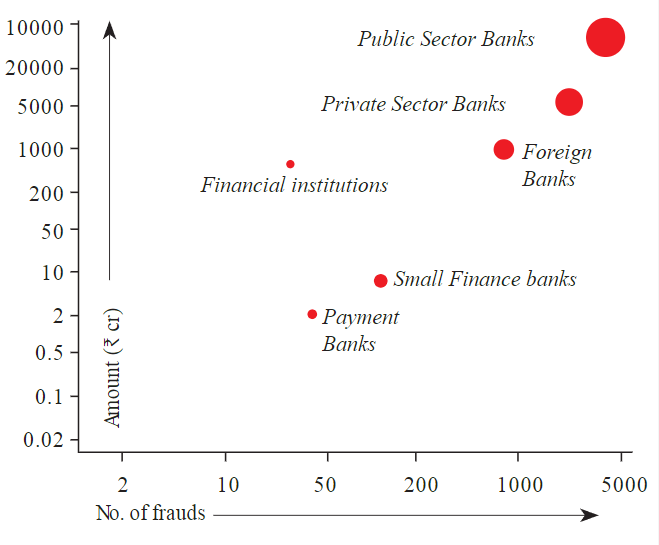
\includegraphics[width=0.7\textwidth]{Figure1.png}\\
\caption{Online Frauds by amount}{Source: The Hindu.}
\label{fig:Figure 1}
\end{center}
\end{figure}

Even though consumers and businesses are getting more comfortable with navigating the digital world, fraudsters are becoming just as adept at finding ways to take advantage of these online trends. According to the Javelin 2021 Identity Fraud Study: Shifting Angles, there was \$56 billion in combined losses from identity fraud & identity fraud scams in 202, accompanied by a significant increase in identity theft scams.

Another fraud management trend pertains to digital wallets and peer-to-peer (P2P) payments. Identity fraud scams claimed 17.5 million digital wallet and P2P fraud victims. Victims of stimulus-refund-related fraud, unemployment money mule scams, and identity fraud scams all owned digital wallets like Apple Pay and Samsung Pay, and P2P products like PayPal, Square and Zelle. 

Feedzai's Quarterly Financial Crime Report, analysing over 12 billion transactions, identifies trends in spending and in fraud attempts to show that this past quarter, as consumer activities increased, fraudsters attempted to hide their fraudulent transactions in legitimate banking. In fact, combining all banking fraud  – internet, telephone, and branch – attacks grew a whopping 159\% in Q1 2021 compared to Q4 2020. 

Online banking made up 96\% of all banking transactions and it accounted for 93\% of all fraud attempts in Q1 2021. This leaves in-branch and telephone banking to make up the remaining 4\%. And while the numbers are smaller, in-branch banking did increase by 442\% this quarter compared with the last as a result of eased lockdown restrictions as businesses begin to open for trade. In addition, telephone scammers upped their efforts and the report shows a 728\% increase in telephone banking fraud.

\subsubsection{Methods of Online Frauds}
Following are some of the most common ways of online frauds in the recent time. Most of the victims are poor users of E-banking and easily believe someone posing as a bank official.
\begin{itemize}
    \item Phishing.
    \item Spam.
    \item Spyware.
    \item Card Skimming.
    \item ATM Skimming.
    \item Hacking.
    \item Identity theft.
\end{itemize}

\subsubsection{Challenges in Fraud Detection}
To detect a potential banking fraud is not an easy task. Some of the challenges faced during fraud detection are:
\begin{itemize}
    \item \textbf{Changing fraud patterns over time - }This is one of the sturdiest to address as fraudsters are always on a lookout for advanced ways to trick the system. This requires the fraud detection programs to be updated with the evolved patterns which decreases its efficiency.
    \item \textbf{Class Imbalance - }More or less, only a small fraction of customers have fraudulent intentions which introduces an imbalance in the classification of fraud detection models. The side effect being a penurious experience for genuine customers, since catching the fraudsters usually involves declining some legitimate transactions.
    \item \textbf{Model Interpretations - }This limitation is associated with the concept of comprehension since models typically give a score indicating whether a transaction is likely to be fraudulent or not — without explaining why.
\end{itemize}
\pagebreak
\subsection{Project Objective}
Cybercrime is one of the major problems faced by the countries across the globe these days. It includes unauthorized access of information and break security like privacy, password, etc. of any person with the use of internet. With the increasing demand of online payment in almost every sector of business, online frauds need to be addressed sternly. 

The vision of this project is to make online banking a safe and secure payment medium through the employment of identity validation. Identity validation is an important requirement in most processes and procedures, whether offline or online. Identity validation lays down trust in the consumer that his funds are being handled fairly. It proves that there is a real person behind the process and is indeed the one he or she claims to be. It is a simple procedure which could keep one's account safe and at the same time, not derange genuine customers as it only takes a couple of moments to complete the whole validation process. Although simple, it is very sound as the command rests solely in the hands of the account holder.

According to Harry (2002), hackers and crackers directly attack servers to commit cybercrimes such as stealing passwords, credit card information and other confidential or secret information; to intercept transactions and communications and commit online frauds\cite{Project_Objective}. Therefore, theft of credentials of users is the major problem to be looked into to solve online frauds. A simple technique of identity validation can save someone from online theft in case his or her credentials get stolen.

\vspace{1cm}
\textbf{Major Objectives}
\begin{itemize}
    \item To create a safe payment gateway for online transactions.
    \item To implement photo verification as a type of identity validation.
    \item To fend off fraudsters from misusing customer's credentials to commit online crimes.
    \item To allow the user to change his/her password in case of suspicious activity on the account.
    \item To place the complete control of a user's online funds into his/her own hands.
\end{itemize}

\vspace{1cm}
Although the main goal of the project is photo verification to validate a transaction, the user is also allowed to change his login credentials in case of detection of hacking or potential theft.

\pagebreak

\subsection{Methodology}
The steps given below provide the solution to the problem of online frauds using identity validation. The solution involves verification of the transactor by the end user in real time and the ability to change the password in case of suspected foul play.
\subsubsection{Photo Verification(Working)}
\begin{enumerate}
    \itemsep0em
    \item User logs into the account who can be a genuine user or a fraud.
    \item The transaction details are entered.
    \item The web app takes a picture of the transactor and sends it on the account holder's email.
    \item The end user can then validate the transaction in which case the transaction is carried out normally.
    \item The end user can deny the transaction which cancels the payment process and the user can also change his account password in case of a suspected fraud.
\end{enumerate}

The above process can be completed in nearly the same time as a normal transaction to conserve the genuine user's time.
\vspace{1.5cm}

\begin{figure}[H]
\begin{center}
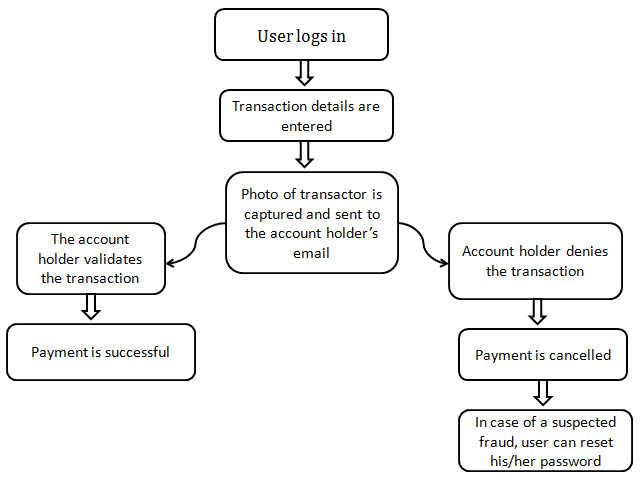
\includegraphics[width=0.8\textwidth]{Figure2.png}\\
\caption{Methodology}
\label{fig:Figure 1}
\end{center}
\end{figure}



\pagebreak

\subsection{Scope of the Project}
Online scams affect a wide range of industries, services and the public in general. There are a large variety of online scams including money theft, identity theft crimes, accessing sensitive information, etc,. 

This project provides a wide range of applications and with slight modifications, finds scope in profusely many areas.\\
\textbf{Some of the areas carrying scope for this project are listed below.}

\subsubsection{Scope in Online Banking}
This project finds its principal application in securing online banking. In case of a theft of a user's login credentials, the thief can run off with the user's online funds. But with photo verification before transaction, the user will be notified of such an attempt of robbery and will have the power to seize control of his account by changing his credentials.
\subsubsection{Scope in protection against data theft}
Theft of sensitive data is another concern of many organisations and even public individuals. Organisations could have varied amounts of data about their products, employees, etc,. with high level of confidentiality. Such data banks are prone to online attacks for illegal access or tampering. Using photo validation in such data banks, the corresponding company officials would always be notified during any potential data breach and would have full control on providing access to the information.
\subsubsection{Scope in Identity theft cases}
Identity theft is a serious case of online scam where a fraud commits online crimes, while identifying as someone else. This project could be moulded to serve as a useful method to put a stop to identity theft in many areas of the internet. This system could be deployed on login pages of sites with high identity theft cases. When a scammer, imposing as someone else tries to login, the app takes a picture and sends it to the email of the account holder who can then verify whether his credentials are being put to misuse. After a scam is discovered, the user can change his credentials to secure his account. 

\pagebreak

\subsection{Project Organisation}
\vspace{1cm}
\subsubsection{Team Members}
\begin{enumerate}
    \itemsep0em
    \item \textbf{Harsh Bokan(12011009, CSE)}
    \item \textbf{Akshdeep Singh(12011026)}
    \item \textbf{Karanbir Singh Pannu(12011011)}
\end{enumerate}

\subsubsection{Technologies Used}
\begin{enumerate}
    \itemsep0em
    \item Google Meet(To work from remote locations)
    \item Canva
    \item GitHub
    \item \LaTeX
\end{enumerate}

\subsubsection{Workflow}
All the three team members worked remotely in this project. GitHub and Google meet proved very handy in cooperating with one another to the end of the project. This project called for a substantial command over both front-end and back-end web designing combined with certain techniques specific to this project. The exploration left us with extensive knowledge to determine the adaptability and flexibility of the project and even to dictate further research in the similar field. The workload was evenly distributed among the team members for efficacious direction of the project.

\subsubsection{Timeline}
The first week was dedicated to discovering an optimal method for the mitigation of online frauds. The following few weeks were devoted to understand the operation of back-end web development, mainly Nodejs, express, database management and photo capture. The major problems involving online frauds were also kept in prime consideration. Apart from these, the knowledge of VS Code and GitHub was key to implement the above tools and collaborate conveniently.
\pagebreak


\subsection{Summary}
\begin{itemize}
    \item \textbf{Purpose/Objective - }Online frauds and scams have become a problem of serious concern with the ever increasing frequency of online payments in almost every part of expenditure and service. These scams have caused the theft of enormous amount of currency and data from organisations and the general public. The motive of this project is to provide a safe and trustworthy gateway of online transactions where the end user gets notified every time his or her account is accessed, with photo identity and  carries the power to validate all the payments. This project will enable customers to safeguard their online funds against potential scams and thefts.
    \item \textbf{Design/Methodology/Approach - }The methodology of the project is plain sailing but fruitful in solving the concerned problem. The project includes a web application where a user logs into a bank account with the particular credentials. On entering the payment gateway, he or she enters the transaction details to execute the payment in someone's favor. Then the transactor is required to submit his/her picture through the web app which would be sent to the account owner via an email. The account owner, with the photo identity of the transactor, can then decide whether to allow or deny the ongoing transaction with a link in the email. If the owner validates the payment, the transaction is carried out successfully, otherwise it is cancelled. The owner is also provided with a link where he/she can reset their account password in case of an unauthorized attempt of access.
    \item \textbf{Scope of Project - }This project is designed for the foremost purpose of preventing scams in banking transactions using the online medium. In case of theft of a user's credentials, this project could help provide the owner with the identity of the thief. However this project could be shaped further to allow the end user to seize his/her account in case of a theft and also report the authorities of the same with a possible identity of the fraudster. This project can also be applied in data security to prevent unauthorised access or modification of data of an organization or individual. This project will incite further research in protection of users' data with the use of advanced technologies like ML and AI to provide facilities like real time document validation, etc.
    \item \textbf{Mitigation of Online Frauds - }With the help of this project, many people with deceitful intentions would be discouraged from tinkering with anyone's property, as they would be required to disclose their identity which could be used against them in a criminal proceeding. It also eliminates the threat of breaches by bots or viruses because they would have no facial identity to produce for the validation of the transaction. 
\end{itemize}
\pagebreak

%Chapter 2
\begin{Large}
\begin{center}
\textbf{CHAPTER\\
\section{STUDY AND REVIEW OF LITERATURE}}\\
\line(1,0){300}\\
\end{center}
\end{Large}
\vspace{0.5cm}
\subsection{Introduction}
The purpose of this chapter is to bring forth some outlines to solve the concerned problem of this project i.e., online frauds. The provided outlines include both, the practices which are currently being used in prevention of scams and those theorised but not yet put into effect.

Online scams impact a vast variety of organizations and services, due to the immense employment of online payments in said services. The different techniques mentioned target online frauds in specific areas and provide the corresponding solution. As the potency of an online scam could vary among different regions of target, the methods laid down could vary in their ability of decreasing the threat of an online fraud.

It should be noted the prime area of focus of this report is the problem of online stealing or banking frauds by misusing a customer's credentials, therefore the problems of identity theft, online harassment, ATM skimming for physical theft, etc,. are not as deeply explored.

The purpose of this chapter is to provide an outline of the different techniques that can be brought to use to diminish the threat of online fraud and not the detailed study of the said techniques. However, these techniques could be studied in detail following the references which provide the bedrock for this project.

This chapter is not limited to only one area of research in the field of online scams, because unlike before, a large number of systems have been made available to the common online servicing platforms, even those requiring high computing power, thanks to the evolution in technology. Many techniques followed in offline validation are now being taken advantage of in the online mode as well.

As this report mainly focuses on online banking frauds, the techniques in this chapter are given only an introduction since there is already a detailed literature on the provided methods.

This chapter is essentially made from a vast number of references from numerous sources which can be further explored to dig deeper in the listed tactics.
\pagebreak

\subsection{Prevailing methodologies used to prevent Online frauds}
\vspace{0.5cm}
\subsubsection{Questionnaire in survey}
Fraudulent behaviors have been predicted by the inconsistent answers provided by the participants\cite{PrevailingMethods1}. The survey conducted by a software checks for proper/consistent answers while it contains some strange or personal questions about social desirability and at the same time collects paradata of the subject(timestamp on questions, movement of mouse, etc,.). This method can detect bots, assess personality traits associated with possible fraudsters, however there is some ethical issues on whether this information should be released or not. The survey would be hard to abandon or resubmit once started, and order of questions would be shuffled with each administration. The survey can further be used to collect IP addresses of devices used to detect encryptions, frequency of survey by one device and also ban IPs of confirmed fraudsters from participating. The cons being that subjects could skip the survey due to discomfort and it only makes frauds difficult and does not prevent them.

\subsubsection{Hidden Markov Model}
The Hidden Markov Model(HMM) is a statistical model in which the system being modeled is assumed to be a Markov model\cite{PrevailingMethods2}. The ranges of transaction amount and types of items are fed to the HMM as observation symbols and states respectively. It is based on the baum-welch algorithm and is initially trained with the normal behavior of account holders. If an incoming transaction is declared fraudulent by the HMM model with high probability, a One Time Password(OTP) is sent to the mobile number for verification. The accuracy of this system was calculated to be around 72\% over a wide variation of input data.


\subsubsection{Fraud Detection Based on Local and Global Behavior}
This research\cite{PrevailingMethods3} provides a system for online fraud detection in real time using two complementary techniques. First is the differential analysis approach which compares account usage to normal history of the user and any deviation would indicate a potential fraud. Second is the global analysis approach where each device is monitored and classified either as legitimate or fraudulent. The model keeps an eye for suspected behavior as large number of accounts accessed by a single fraudster, small transactions made in many accounts, increased number of password failures before a fraud. It maintains a suspect list which contains devices with fraudulent behaviors. These list items are then explicitly deemed as genuine or fraudulent. The effective identification is made by a component installed on every device during its first access to the bank. A monitor counts the number of different accounts accessed by each device and the data collected is used by the global analysis module to predict the possibility of a transaction being a fraud.

\subsubsection{Using financial intelligence to target fraud victimisation}
This study\cite{PrevailingMethods4} based in Australia explains the emergence of a victim oriented approach to target online frauds, where police and consumer protection agencies put financial intelligence at work to identify potential online fraud victims. Operation Sunbird(2012) targeted advance fee frauds and romance fraud victimisation where a victim sends a small amount of money hoping to receive a larger sum in return. It is a five stage process. First stage is intelligence where WAPOL(West Australian Police) use intelligence to find potential victims by screening potential transactions. Second stage is intervention where Commerce sends a letter to the household warning the victim of a high possibility of fraud. Third stage is intervention where Commerce liaises with bank to block transactions of both the potential fraud and victim. Fourth stage involves intelligence where Commerce gathers and analysis intelligence gathered by investigation and letter recipient who made contact. The final stage is investigation whereby WAPOL apprehends possible suspects and refers the intelligence of corresponding countries about the fraud.

\subsubsection{Hierarchical attention mechanism}
This study\cite{PrevailingMethods5} puts to use, an attention based classifier for real time risk assessment of each individual transaction in the form of a fraud probability. This mechanism consists of two main components. First component entails embedding of categorical features in a continuous space and uniting those characteristics into one vector using an attention mechanism. The second component is responsible to expose fraudulent activity carried out by a sequence level attention. Tested over 26.1 million transactions over six months, this model outperformed LSTM(Long Short-Term Memory) proving  that there is substantial benefit in attention based models that dynamically assign weights to transactions.

\subsubsection{Embedded Training Email System}
Phishing attacks involve criminals disguise as legit websites to lure users into providing their personal information or releasing some malware into their system. This study\cite{PrevailingMethods6} deals with training people about phishing attacks. Users are communicated to a website through periodic emails which could be a potential phishing attempt, and then they are tested whether they would disclose their information or not. The medium of email is chosen as most of phishing attacks occur through email. The study also explains the development of a game-based approach to train people to identify phishing sites.

\pagebreak

\subsection{Summary}
This chapter brings forward the available and theorised technologies used to detect and prevent online frauds. The methods mentioned have been taken different researches carried out for online fraud prevention.

Online theft and crimes is a very vast field and is understudied in many respects. It impacts the society at many points and demands serious attention. These studies are based on the different areas of impact of online fraudsters and therefore a different degree of efficiency in their execution. 

The purpose of this chapter is to lay out a thorough but not all-inclusive review of the literature of the different techniques discussed. However these studies could be investigated further through the reference provided at the end. 

The methodologies presented in this chapter communicate many ways for the prevention of online scams ex, survey through questions to detect fraudulent behavior, analysing behavioral patterns of devices and users accessing customer's account to find out any suspicious activity through HMM, local and global behavior, hierarchical attention, etc,. Methods of educating the users against such potential crimes and monitoring and helping victims were also discussed as mitigation techniques. 


\pagebreak

\begin{thebibliography}{}
\bibitem{Project_Objective}
Shewangu Dzomira, Ph.D., Department of Finance, Risk Managementand Banking, College of Economics & Management Sciences, Univer-sity of South Africa, South Africa.
\bibitem{PrevailingMethods1}
Teitcher, J. E., Bockting, W. O., Bauermeister, J. A., Hoefer, C. J., Miner, M. H., & Klitzman, R. L. (2015). Detecting, preventing, and responding to "fraudsters" in internet research: ethics and tradeoffs. The Journal of law, medicine & ethics : a journal of the American Society of Law, Medicine & Ethics, 43(1), 116–133. https://doi.org/10.1111/jlme.12200
\bibitem{PrevailingMethods2}
Mhamane S, Lobo L.M.R.J. Use of Hidden Markov Model as Internet Banking Fraud Detection, International Journal of Computer Applications (0975 – 8887), Volume 45– No.21, May 2012
\bibitem{PrevailingMethods3}
Kovach, Stephan & Ruggiero, W.V.. (2011). Online Banking Fraud Detection Based on Local and Global Behavior. In: Proc. of the Fifth International Conference on Digital Society.
\bibitem{PrevailingMethods4}
Cassandra Cross (2016) Using financial intelligence to target online fraud victimisation: applying a tertiary prevention perspective, Criminal Justice Studies, 29:2, 125-142, DOI: 10.1080/1478601X.2016.1170278
\bibitem{PrevailingMethods5}
Achituve, Idan & Kraus, Sarit & Goldberger, Jacob. (2019). Interpretable Online Banking Fraud Detection Based On Hierarchical Attention Mechanism. 1-6. 10.1109/MLSP.2019.8918896. 
\bibitem{PrevailingMethods6}
Cranor P.K.L, Hong Y.W.R.J, Nunge A.A.E.(2006) Protecting People from Phishing: The Design and Evaluation of an Embedded Training Email System, CyLab Carnegie Mellon University Pittsburgh(November 9, 2006)
\end{thebibliography}

\end{document}